/section{Zielsetzung}
In diesem Versuch sollen mithilfe der Tomographie mit Gamma-Strahlung verschiedene Würfel auf ihre Zusammensetzung untersucht werden.
Der Fokus liegt dabei auf das Verständnis von Gamma-Strahlung und die Funktionsweise des Szintillationsdetektors.

\section{Theorie}
\label{sec:Theorie}

\subsection{Tomographie}
Die Tomographie ist ein bildgebendes Verfahren.
Wird ein Objekt untersucht, können zwei dimensionale Bildschnitte erzeugt werden um diese zu untersuchen.
Trifft Strahlung auf Materie, wird diese durch Wechselwirkungen abgeschwächt.
Dabei ergibt sich für die Ausgangsintensität $I_\text{aus}$ folgender Zusammenhang:
\begin{equation}
    I_\text{aus} = I_0 \cdot \exp{(- \sum_{i} \mu_i d_i)} \, .
\end{equation}
$I_0$ beschreibt die Eingangsintensität, $\mu_i$ den Absorptionskoeffizienten und $d_i$ die zurückgelegte Strecke nach Strahlrichtung i.
Sind Eingangs- und Ausgangsintensität bekannt, kann durch logarithmieren ein Ausdruck für den Absorptionskoeffizienten/Abschwächungskoeffizient? aufgestellt werden:
\begin{equation}
    \label{eqn:SUMME}
    \sum_{i} \mu_i d_i = \ln{I_\text{aus}/I_0} \, .
\end{equation}
Durch die Messungen entsteht ein lineares Gleichungssystem, sodass \eqref{SUMME} in Matrixschreibweise dargestellt werden kann:
\begin{equation}
    \label{eqn:matrix}
    \symbf{A} \mu = I \, ,
\end{equation}
wobei für $I = \ln{I_\text{aus}/I_0}$ gilt.
Die Matrix A beschreibt die Messungen.
Das entstandene LGS muss überbestimmt sein.
Also darf die $\symbf{A}$ A nicht singulär sein, so können die Werte für die Absorptionskoeffizienten mit dem Verfahren für die kleinsten Quadrate gefittet werden.
Mit Multiplikation mit $\symbf{A}^\top$ ergibt sich folgender Ausdruck für den Absorptionskoeffizienten $\mu$
\begin{equation}
    \mu = (\symbf{A}^\top \cdot \symbf{A})^{-1} \cdot \symbf{A}^\top \cdot I \, .
\end{equation}

\subsection{Projektionen}
Um keine singuläre Matrix A zu erhalten, werden die in \autoref{fig:Projektionen} gezeigten Projektionen für die Messungen verwendet.
Insgesamt gibt es 12 Projektionsrichtungen.

\begin{figure}[H]
    \centering
    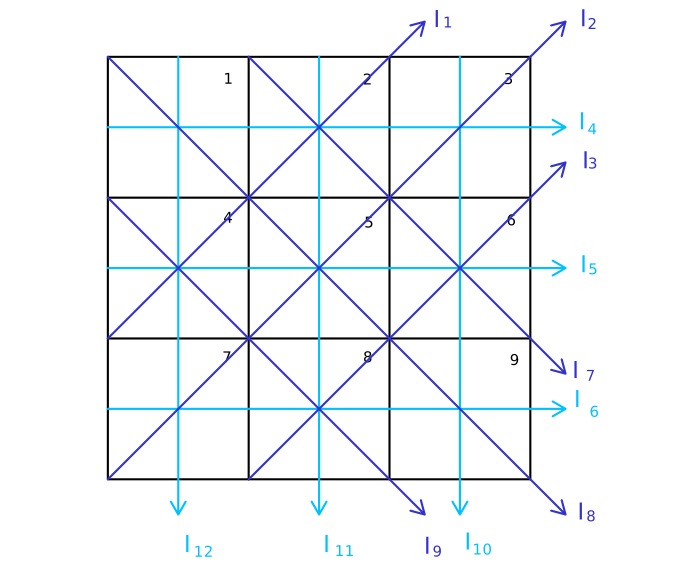
\includegraphics[width=\textwidth]{bilder/projektionen.png}
    \caption{Schematischer Aufbau der verwendeten Projektionen.}
    \label{fig:Projektionen}
\end{figure}

\subsection{Absorptionsphänomene}
Da Gamma-Strahlung verwendet wird, wird im Folgenden auf die Hauptwechselwirkungen eingegangen.
Die drei wichtigsten Effekte, die bei Photon-Materie Wechselwirkungen auftreten, sind Photoeffekt, Comptoneffekt und Paarbildung.
\begin{itemize}
    \item   Photoeffekt: Wenn ein Photon mindestens eine Energie hat, die so groß ist wie die Bindungsenergie eines Elektrons, dann kann das Elektron durch Aufnahme der Photonenenergie das Atom verlassen.
    
    \item   Comptoneffekt: Dieser Effekt beschreibt einen elastischen Stoß zwischen Photon und Elektron.
            Das Photon wird an einem Elektron gestreut und gibt dabei einen Teil seiner Energie ab.
            Es hat nach dem Stoß eine andere Wellenlänge. Wichtig ist, dass nach dem Stoß das Photon weiter existiert.
    
    \item   Paarbildung: Wenn die Energie eines Photons die Energie eines Elektron-Positron Paares entspricht, kann sich dieses Photon in diese beiden Teilchen aufteilen.
            Dazu muss es auch in der Nähe des Atomkerns sein, welches als Stoßpartner fungiert. 
    
\end{itemize}

In diesem Versuch sind die beobachtbaren Effekte der Compton und Photoeffekt.
Da die Energie der Gamma-Strahlung bei $\SI{600}{\kilo\electronvolt}$ liegt, kommt es zu keiner Paarbildung.
Die dafür benötigte Energie muss bei $2 \cdot \SI{511}{\kilo\electronvolt}$ liegen.

\subsection{Absorptionskoeffiziente}
Da die Untersuchung der Würfel bzw. die Materialbestimmung über die Ermittlung der Absorptionskoeffizienten läuft, werden in \autoref{tab:lit} die Koeffizienten der möglichen Materialien aufgenommen.
Die ermittelten Absorptionskoeffizienten werden mit den Litaraturwerten verglichen um so auf das Material im jeweiligen Würfel zu schließen.

\begin{table}
    \centering
    \caption{Die Literaturwerte des Massenschwächungskoeffizienten $\sigma$ , der Stoffdichte $\rho$ und dem Absorptionskoeffizienten $\mu$ der mögliche Materialien.}
    \label{tab:lit}
    \begin{tabular}{c S[table-format=2.3] S[table-format=2.2] S[table-format=1.3]}
        \toprule
        {Stoff} & {$ \sigma \mathbin{/}  \left(\SI{e-2}{\centi\metre\squared\per\gram}\right)$\cite{massenbumms}} & {$\rho \mathbin{/}  \left(\si{\gram\per\centi\metre\cubic}\right)$\cite{dichten}} & {$\mu \mathbin{/} \left( \si{\per\centi\metre\cubic}\right)$} \\
        \midrule
        Aluminium & 7.802   & 2.7   & 0.211 \\
        Blei      & 12.48   & 11.34 & 1.415 \\
        Eisen     & 7.704   & 7.87  & 0.606 \\
        Messing   & 7.651   & 8.4   & 0.642 \\
        Delrin    & 8.6     & 1.42  & 0.121 \\
        \bottomrule
    \end{tabular}
\end{table}